\section{Negative results}
\label{sec:negative}

\paragraph{Checkpoint selection without labels.} We tested six signals for choosing a
checkpoint without target labels, scoring each by the TPR it loses against the best checkpoint
on the development fold, over nine development runs. Source-validation AUROC and purity
saturate from the first checkpoint and carry no information. The norm of the head's gradient,
proposed as a model-internal diagnostic~\citep{headgradnorm}, points in opposite directions on
different methods. All but one signal fell inside the range
of a random choice around our rule of taking the last checkpoint. The exception,
source-validation TPR, was the best selector on one unfrozen run and the worst on the other,
and nothing without labels tells the two cases apart, so we kept the last checkpoint. These are
development-fold values on the original test pool, and three of the signals could not be
computed on the unfrozen runs because their per-checkpoint files were lost.

\paragraph{Budget peak and decay onset are unmeasurable.} On the development fold the peak of
the FreeMatch curve cannot be located, since the steps within two positives of the best are
spread from \rwFzStepMin{} to \rwFzStepMax{}, and the onset of decay is detectable only at the
8000-step cap (Table~\ref{tab:orderings2}, rows 1 and 2). Appendix~\ref{sec:budget-detail}
describes how we fixed each budget instead.

\paragraph{The memorisation diagnostic is inconclusive.} Each fold's target pool holds about
782 images, few enough for an unfrozen encoder to memorise. We pre-declared a diagnostic: the
gap in a nuclear-norm statistic between a target slice an arm trains on and the held-out slice.
On BNM the gap resolves under one declared reading and not under the reading we declared
primary. On the $\lambda=0$ control, where neither slice is trained on, its scatter is larger
than the effect it is meant to bound. CORAL and FreeMatch have no held-out slice. DANN and its
control share one and differ only in $\lambda$; computed on their stored checkpoints in a
retrospective analysis whose rule we declared before computing it, DANN's gap minus the control's is
$\mzPrim{}$ $[\mzPrimLo{}, \mzPrimHi{}]$ at the read-off step and, as the secondary reading,
$\mzSec{}$ $[\mzSecLo{}, \mzSecHi{}]$ averaged over checkpoints (Table~\ref{tab:dl-memorisation});
both intervals are without multiplicity correction and probably too narrow, because the folds'
target pools overlap (Section~\ref{sec:intervals}).
Re-drawing the random augmentation of the same images moved one fold's gap by
$\mzViewShift{}$, as large as the effects the diagnostic is meant to detect, so we computed these
values without augmentation. They are not comparable with BNM's gap, which used one
augmented view per image. Whether part of the adaptation gain comes from fitting these
particular images therefore remains undetermined.

\paragraph{Our predictions for the dilution experiment.} Most components of the \dlNPredWord{}
predictions we recorded before the 1:10 runs failed; Section~\ref{sec:results-dilute} scores them.

\begin{figure}[t]
\centering
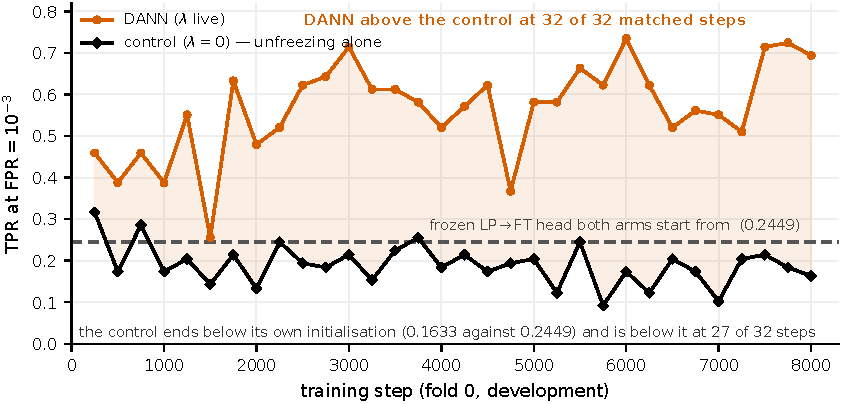
\includegraphics[width=\textwidth]{F4_fold0_curves.pdf}
\caption{\textbf{The $\lambda=0$ control and DANN on the development fold}, identical at step 0
and differing only in $\lambda$. The dashed line is the frozen linear-probe head both start
from. The control ends below it. One fold; it enters no headline number.}
\label{fig:fold0}
\end{figure}
